% !TEX encoding = UTF-8 Unicode
% !TEX TS-program = LuaLaTeX
% !TEX root = ../memoire.tex
% !TEX spellcheck = fr-FR

%************************************************
\chapter{Données déséquilibrées}
\label{chap:cinq}
%************************************************


%\citet{Dupret2001}
%\citet{Lopez2014}
%\citet{Zhai2011}
%\citet{Zhou2012a}
%\citet{Gao2015}
%\citet{Nikulin2009}
%\citet{Dong2011}

Le principal obstacle dans la classification en scoring est le déséquilibre souvent très important entre la classe d'intérêt et la classe majoritaire. Ce déséquilibre a pour conséquence de biaiser la performance du classifieur vers la classe majoritaire au détriment de la classe minoritaire puisqu'il n'est pas rare d'observer des ratios de $99$\% contre $1$\% dans le milieu du credit scoring par exemple. Il est donc primordial de mettre en place des méthodes visant à améliorer les performances réelles du classifieur en présence de classes déséquilibrées.

\section{Sous-échantillonnage}

Une première méthode possible pour réduire le déséquilibre entre les classes est tout simplement de supprimer un certain nombre d'observations de la classe majoritaire pour se ramener à une distribution plus équilibrée. Une simple suppression aléatoire de données majoritaires est possible, mais présente l'inconvénient extrêmement pénalisant d'ignorer la majorité des données lors de la construction du modèle. Cette perte d'information peut conduire à une diminution des performances qui serait assez importante pour ne pas contrebalancer le gain amené par le rééquilibrage. Il convient donc d'introduire des méthodes plus intelligentes qui évitent de supprimer l'information utile.

\subsection{Sous-échantillonnage informé}

\begin{definition}[Liens de Tomek]
    Soit $x$ et $y$ deux individus de classes différentes et soit $d : \mathcal{X} \times \mathcal{X} \rightarrow \mathbb{R}^+$ une distance sur les individus.
    $(x,y)$ est appelé lien de Tomek si $\nexists z , d(x,z) < d(x,y) \text{ ou } d(y,z) < d(x,y)$. Autrement dit si $x$ et $y$ sont plus proches voisins.
\end{definition}

Il est alors possible de sous-échantillonner en supprimant tous les individus de la classe majoritaire membre d'un lien de Tomek.

\begin{definition}[\ac{cnn}, \cite{Hart1968,Kubat1997}]
    Le but est la construction d'un sous-ensemble consistant au sens de \citet{Hart1968}. Tout d'abord un ensemble $\mathcal{L'}$ contenant tous les individus de la classe minoritaire et un individu de la classe majoritaire tiré au hasard est construit, puis la règle de classification $1$-NN est utilisée pour classifier tous les individus. Chaque individu mal classé est ajouté à $\mathcal{L'}$ et la procédure est répétée jusqu'à ce qu'il n'y ait plus d'individus mal classés.
\end{definition}

\begin{definition}[\ac{enn}, \cite{Wilson1972,Laurikkala2001}]
    Pour chaque $\mathbf{x}_i$ ses trois plus proches voisins sont recherchés. Si $\mathbf{x}_i$ appartient à la classe majoritaire et est mal classé par ses voisins alors celui-ci est supprimé. S'il appartient à la classe minoritaire et est mal classé, alors ses trois voisins sont retirés.
\end{definition}

\begin{definition}[\ac{oss},\cite{Kubat1997}]
    La méthode \ac{oss} est la combinaison des liens de Tomek suivi de \ac{enn}. Ainsi les individus considérés comme \emph{bruyants} sont retirés par l'élimination des liens de Tomek puis les individus à la frontière par \ac{enn}. Il est également possible d'effectuer l'opération dans l'autre sens tel que proposé par \citet{Batista2004}.
\end{definition}

Ces méthodes de rééquilibrage procèdent à une forme de régularisation a priori de la surface de séparation en supprimant les exemples les plus à même de grandement modifier la surface. On comprend pourquoi il est légitime d'espérer une amélioration de l'erreur de généralisation.

Les résultats de \citet{Chen2004,Japkowicz2000} semblent indiquer un fort potentiel de ces techniques pour les données purement théoriques mais toutes ces méthodes utilisent à une étape la distance entre les individus. Une telle distance est difficile à définir dans le cas des données hétérogènes et diminue fortement les performances que l'on obtient en pratique. Nous introduisons dans~\ref{distances} des distances adaptées à nos données pour essayer de résoudre ce problème.

\subsection{Balanced et Roughly Balanced Random Forest}

Le sous-échantillonnage naïf provoque une perte d'information trop importante, mais les forêts aléatoires présentent déjà une procédure de sous-échantillonnage à travers le \ac{bagging}; il est donc possible d'adapter le \ac{bagging} afin de rétablir l'équilibre des classes.

La première méthode proposée par \citet{Breiman2001} est la méthode \ac{brf} qui consiste à effectuer le tirage bootstrap sur l'échantillon d'observations de la classe minoritaire et celui de la classe majoritaire de manière indépendante. Ainsi si l'on note $\mathcal{L}_m$ les individus de la classe minoritaire et $\mathcal{L}_M$ ceux de la classe majoritaire on construit l'échantillon bootstrap pour chaque arbre en tirant $\vert \mathcal{L}_m \vert $ individus de $\mathcal{L}_m$ avec remise et le même nombre d'individus de $\mathcal{L}_M$. Ainsi chaque arbre est construit sur un échantillon de taille $2  \vert \mathcal{L}_m \vert$ très réduit, mais parfaitement équilibré. Contrairement au sous-échantillonnage naïf où la perte d'information est dommageable ici le sous-échantillonnage a lieu à chaque arbre, mais tout l'échantillon est considéré pour la forêt. Ainsi, quitte à augmenter le nombre d'arbres, il n'y a pas de perte d'information.

Une version modifiée de cet algorithme est l'algorithme \ac{rbrf} introduit dans \citet{Hido2009b}. Ici la procédure de \ac{bagging} est répliquée en ajoutant un a priori sur la distribution des classes afin éventuellement de mieux capturer les avantages du \ac{bagging} pour les forêts aléatoires. On tire toujours $\vert \mathcal{L}_m \vert $ individus bootstrap de $\mathcal{L}_m$ mais le nombre d'individus tirés dans $\mathcal{L}_M$ est aléatoire. On tire alors $ \mathrm{BN} ( \vert \mathcal{L}_m \vert , 0.5 ) $ individus de $\mathcal{L}_M$ où $\mathrm{BN}(n,q)$ est la loi binomiale négative avec $n$ le nombre d'échecs et $q$ la probabilité d'échec.

En effet la procédure de bootstrap tire chaque point $(x,y) \in \mathcal{L}$ avec probabilité $p(x,y)$. En utilisant la formule de Bayes on a $p(x,y) = p(y) p(x \mid y )$. Sous cette décomposition, tirer un échantillon bootstrap revient à d'abord tirer $n_y$ sous la loi binomiale $\mathrm{B} ( \vert \mathcal{L} \vert , p(y) )$ puis $n_y$ individus de la classe $y$ sont tirés uniformément. \todo{faire la preuve de l'équivalence de ces tirages.} Il est alors possible de choisir l'a priori $p(y) = 0.5$ pour effecteur le tirage. Cela revient donc à chaque tirage, à sélectionner avec probabilité $p(y) = 0.5$ la classe puis à choisir uniformément un individu au sein de celle-ci. Puisque le nombre d'individus minoritaires est faible, on ajoute une seconde restriction en arrêtant le tirage une fois que $\vert \mathcal{L}_m \vert$ individus de la classe minoritaire ont été tirés, ce qui revient à choisir le nombre d'individus à tirer selon une loi binomiale négative. \todo{POURQUOI?}

\begin{figure}[htbp]
    \makebox[\textwidth][c]{
    \begin{tikzpicture}
    \begin{axis}[name= plot1, domain=0:1, ymin=0, ymax = 1, enlargelimits = false, xlabel = {Taux de faux positifs}, ylabel = {Taux de vrais positifs}, legend style={draw=none,legend pos=south east}]
            \addplot[no markers, const plot, blue] table [x = "fpr", y = "tpr", col sep = comma] {images/roc_rbrf.csv};
            \addlegendentry{RBRF}
            \addplot[no markers, const plot] table [x = "fpr", y = "tpr", col sep = comma] {images/roc_rf.csv};
            \addlegendentry{RF}
            \addplot[no markers, black, dashed] {x};
    \end{axis}

    \begin{axis}[name = plot2, at=(plot1.right of south east), anchor=left of south west, domain=0:1, ymin=0, ymax = 1, enlargelimits = false, xlabel = {Taux de faux positifs}, legend style={draw=none,legend pos=south east}]
            \addplot[no markers, const plot, blue] table [x = "fpr", y = "tpr", col sep = comma] {images/roc_brf.csv};
            \addlegendentry{BRF}
            \addplot[no markers, const plot] table [x = "fpr", y = "tpr", col sep = comma] {images/roc_rf.csv};
            \addlegendentry{RF}
            \addplot[no markers, black, dashed] {x};
    \end{axis}
    \end{tikzpicture}
    }
    \caption{Performances de BRF ($\mathrm{AUC} = 0.8432$) et RBRF ($\mathrm{AUC} = 0.8452$)}
\end{figure}

Ces deux modifications du \ac{bagging} cherchent, au moins en moyenne, à égaliser les classes. Néanmoins \citet{Dupret2001} montrent qu'un rééquilibrage parfait n'est pas optimal, nous introduisons alors deux variantes des algorithmes précédents.

Si $q_a$ est la proportion d'individus appartenant à la classe $a$ dans l'échantillon d'apprentissage alors on fixe $\alpha$ comme proportion d'individus  de la classe $a$ tirés durant le bagging:
\begin{equation*}
    \alpha = \frac{1}{2} + \frac{2 q_a - 1}{4}
\end{equation*}

On introduit alors l'algorithme \ac{nbrf} comme modification de \ac{brf}:
\begin{algorithm}
\caption{Algorithme NBRF pour les forêts aléatoires}
\begin{algorithmic}
    \Procedure{NBRF}{$\mathcal{L}$, règle arrêt, $M$}
    \State{$q_a \gets \frac{\vert \mathcal{L}_m \vert}{\vert \mathcal{L} \vert}$}
    \State{$\alpha \gets \frac{1}{2} + \frac{1 - 2 q_a}{4}$}
    \For{chaque arbre $i < M$}
        \State{$\mathcal{L}_n \gets \vert \mathcal{L}_m \vert$ individus minoritaires et $\vert \alpha \mathcal{L}_m \vert$ majoritaires }
        \For{chaque nœud $j$ et règle d'arrêt non remplie}
            \State{$K$ variables tirées aléatoirements}
            \State{Choix de la meilleur coupure}
        \EndFor
    \EndFor
    \State \Return $\left(\mathrm{Arbres_i}\right)$
    \EndProcedure
\end{algorithmic}    
\end{algorithm}

Afin de conserver l'esprit de l'algorithme \ac{rbrf} on introduit \ac{vrbrf}
\begin{algorithm}
\caption{Algorithme VRBRF pour les forêts aléatoires}
\begin{algorithmic}
    \Procedure{VRBRF}{$\mathcal{L}$, règle arrêt, $M$}
    \State{$q_a \gets \frac{\vert \mathcal{L}_m \vert}{\vert \mathcal{L} \vert}$}
    \State{$\alpha \gets \frac{1}{2} + \frac{1 - 2 q_a}{4}$}
    \For{chaque arbre $i < M$}
        \State{$\mathcal{L}_n \gets \vert \mathcal{L}_m \vert$ minoritaires et $\mathrm{BN} ( \alpha \vert \mathcal{L}_n \vert , 0.5 )$ majoritaires }
        \For{chaque nœud $j$ et règle d'arrêt non remplie}
            \State{Tirer $K$ variables aléatoirements}
            \State{Choisir la meilleure coupure}
        \EndFor
    \EndFor
    \State \Return $\left(\mathrm{Arbres_i}\right)$
    \EndProcedure
\end{algorithmic}    
\end{algorithm}

\begin{figure}[htbp]
    \makebox[\textwidth][c]{
    \begin{tikzpicture}
    \begin{axis}[name= plot1, domain=0:1, ymin=0, ymax = 1, enlargelimits = false, xlabel = {Taux de faux positifs}, ylabel = {Taux de vrais positifs}, legend style={draw=none,legend pos=south east}]
            \addplot[no markers, const plot, blue] table [x = "fpr", y = "tpr", col sep = comma] {images/roc_nbrf.csv};
            \addlegendentry{NBRF}
            \addplot[no markers, const plot] table [x = "fpr", y = "tpr", col sep = comma] {images/roc_rf.csv};
            \addlegendentry{RF}
            \addplot[no markers, black, dashed] {x};
    \end{axis}

    \begin{axis}[name = plot2, at=(plot1.right of south east), anchor=left of south west, domain=0:1, ymin=0, ymax = 1, enlargelimits = false, xlabel = {Taux de faux positifs}, legend style={draw=none,legend pos=south east}]
            \addplot[no markers, const plot, blue] table [x = "fpr", y = "tpr", col sep = comma] {images/roc_vrbrf.csv};
            \addlegendentry{VRBRF}
            \addplot[no markers, const plot] table [x = "fpr", y = "tpr", col sep = comma] {images/roc_rf.csv};
            \addlegendentry{RF}
            \addplot[no markers, black, dashed] {x};
    \end{axis}
    \end{tikzpicture}
    }
    \caption{Performances de NBRF ($\mathrm{AUC} = 0.8427$) et VRBRF ($\mathrm{AUC} = 0.8421$)}
\end{figure}

\todo{Performances pas normales}

\section{Sur-échantillonnage}

De la même façon qu'il est possible de rétablir l'équilibre en diminuant la proportion d'individus de la classe majoritaire, il est possible d'augmenter le nombre d'individus de la classe minoritaire. La méthode naïve consiste alors à tout simplement dupliquer les individus minoritaires, mais le risque de sur-apprentissage augmente alors en conséquence. On peut alors pour diminuer ce risque introduire des méthodes de sur-échantillonnage dites \emph{synthétiques}.

\subsection{SMOTE}

Le principe de SMOTE tel qu'introduit par \citet{Chawla2002a} est simple: augmenter le nombre d'observations minoritaires sans duplication tout en restant dans la zone de l'espace où l'on s'attendrait à trouver de telles observations. Pour cela, ils créent des observations synthétiques en extrapolant entre des observations minoritaires proches déjà présentes. Les observations considérées pour l'extrapolation sont choisies par \ac{knn} et tout simplement linéairement interpolées.

Cette méthode est très simple d'application dans le cas où les variables sont homogènes numériques mais ne peut pas s'appliquer telle quelle à un échantillon hétérogène puisque les notions de distance et d'interpolation ne sont pas bien définies. Le cas de l'interpolation est simplement résolu en fixant un seuil et en décidant par exemple que si $x_i$ est une variable catégorielle alors le nouvel individu synthétique $\mathbf{x}_s$ interpolé à partir de $\mathbf{x}_1$ et $\mathbf{x}_2$ prend comme valeur pour $\mathbf{x}_{s,i}$, $\mathbf{x}_1$ si le coefficient d'interpolation est inférieur à $0.5$, $\mathbf{x}_2$ sinon.

\subsubsection{Borderline-SMOTE}

\citet{Han2005} proposent une modification de SMOTE cherchant à concentrer la création d'individus synthétiques aux zones \emph{frontières} puisque ce sont ceux-ci qui majoritairement détermineront la surface de décision. La modification par rapport à SMOTE est alors de rajouter une étape permettant de décider si un individu minoritaire est à la frontière ou non.
\begin{enumerate}
    \item Pour chaque $\mathbf{x}_i$ de la classe minoritaire on cherche les $k$ plus proches voisins, on note $k_M$ le nombre de ces voisins appartenant à la classe majoritaire.
    \item Si $k_M = k$ alors l'individu est considéré comme du bruit et est sauté, si $k/2 \leq k_M \leq k$ alors $\mathbf{x}_i$ est considéré comme étant à la frontière $F$.
    \item Pour chaque individu de $F$, on construit des individus synthétiques à partir de ses $k$ plus proches voisins dans $\mathcal{L}_1$ en utilisant un coefficient d'interpolation aléatoire compris entre $0$ et $1$.
\end{enumerate}
Les auteurs proposent une autre variante qui, au lieu de ne considérer que les voisins appartenant à $\mathcal{L}_1$, considère tout $\mathcal{L}$. Dans ce cas, si l'interpolation entre $\mathbf{x} \in \mathcal{L}_1$ et $\mathbf{x'} \in \mathcal{L}_0$ se fait à l'aide d'un coefficient aléatoire compris entre $0$ et $1/2$.

\subsubsection{ADA-SYN}

Dans cette variante proposée par \citet{He2008}, le nombre d'individus synthétiques à créer pour chaque individu de la classe majoritaire est pondéré par $\frac{k_M^i}{\sum_{i=1}^{\vert \mathcal{L}_1 \vert} k_M^i}$ où $k_M^i$ est le nombre d'individus de la classe majoritaire présent parmi les $k$ plus proches voisins de $\mathbf{x}_i \in \mathcal{L}_1$

\subsection{Distances hétérogènes}

Dans le cas des données hétérogènes, il est nécéssaire d'introduire de nouvelles métriques. Il en existe de nombreuses \citep{Wilson1997,Lumijarvi2004,Rodriguez2008} mais nous ne donnons ici que deux exemples simples.

\begin{definition}[Distance \ac{heom}]
    On appelle $\mathrm{HEOM}$ la distance définie par $\mathrm{HEOM} (\mathbf{x},\mathbf{x}') = \sqrt{ \sum_{j=1}^p \mathrm{d}_{X_j} (\mathbf{x}_j,\mathbf{x}'_j) }$ avec:
    \begin{align*}
        &\mathrm{d}_{X_j} (x_j,x'_j) = \begin{cases}
            \mathrm{d}_Q (x_j,x'_j) \text{ si } X_j \text{ qualitative} \\
            \mathrm{d}_N (x_j,x'_j) \text{ si } X_j \text{ quantitative}
        \end{cases} \\
        &\mathrm{d}_Q (x_j,x'_j) = \begin{cases}
            1 \text{ si } x_j = x'_j \\
            0 \text{ sinon}
        \end{cases}\\
        &\mathrm{d}_N (x_j,x'_j) = \frac{\vert x_j - x'_j \vert}{\max X_j - \min X_j}
    \end{align*}
\end{definition}

\begin{definition}[Distance \ac{hvdm}]
    On appelle $\mathrm{HVDM}$ la distance définie par $\mathrm{HVDM} (\mathbf{x},\mathbf{x}') = \sqrt{ \sum_{j=1}^p \mathrm{d}'_{X_j} (\mathbf{x}_j,\mathbf{x}'_j) }$ avec:
    \begin{align*}
        &\mathrm{d}'_{X_j} (x_j,x'_j) = \begin{cases}
            \mathrm{VDM}_Q (x_j,x'_j) \text{ si } X_j \text{ qualitative} \\
            \mathrm{VDM}_N (x_j,x'_j) \text{ si } X_j \text{ quantitative}
        \end{cases}\\
        &\mathrm{VDM}_Q (x_j,x'_j) = \frac{1}{2} \sum_{c=1}^J \left\vert \mathbb{P} \left( Y = c \mid X_j = x_j \right) - \mathbb{P} \left( Y = c \mid X_j = x'_j \right) \right\vert^q \\
        &\mathrm{VDM}_N (x_j,x'_j) = \frac{ \vert x_j - x'_j \vert }{4 \mathbb{V} \left[ X_j \right]}
    \end{align*}
\end{definition}

Sur le même principe que \ac{hvdm}, nous introduisons dans~\ref{distances} une distance adaptée à notre cas particulier de la classification binaire.

\section{Fonction de coût}

La plupart des algorithmes de classification cherchent à minimiser l'erreur 0-1, c'est-à-dire le nombre de mauvaises prédictions. Néanmoins dans un grand nombre de cas réels, le coût de mauvaise classification est plus élevé pour une des classes (souvent la classe minoritaire) que pour les autres classes. En effet en prenant par exemple le cas de la classification des mails en Spam ou Non-Spam, mal classifier un mail indésirable en tant que Non-Spam ne coûtera que quelques minutes de votre temps, à l'inverse mal classifier un mail de votre employeur en tant que Spam aura un coût potentiellement très élevé. Il convient alors au lieu de minimiser le taux d'erreur de minimiser le coût à partir d'une matrice de coûts $C$ où $C(i,j)$ est le coût de classification d'un élément de vraie classe $i$ en classe $j$.

\subsection{Weighted Random Forest}

Une première solution pour prendre en compte le coût de mauvaise classification est d'intégrer celui-ci directement à la procédure d'apprentissage des arbres aléatoires. Pour cela \citet{Breiman2001} propose d'attribuer un poids aux observations en donnant un poids plus fort aux classes que l'on souhaite mieux classer, c'est-à-dire celles qui possèdent le plus fort coût de mauvaise classification.
Dans la procédure standard d'induction de l'arbre, l'impureté de Gini d'un nœud est
\begin{equation*}
    i_G = \sum_i p_i ( 1 - p_i ) = 1 - \sum_i p_i^2
\end{equation*}
où $p_i$ est la proportion de l'échantillon du nœud qui appartient à la classe $i$. Dans ce cas l'impureté, est maximale quand la distribution des classes est uniforme, ce qui est implicitement considéré comme la distribution a priori des classes. Dans le cas où les classes ne sont pas uniformes, on veut alors modifier la fonction d'impureté pour refléter ce déséquilibre et placer le maximum d'impureté à la distribution a priori des classes. Si l'on note $w_i$ le poids de la classe $i$ et $n_i$ le nombre d'observations de $i$ dans le nœud fils $t_R$ alors le poids total dans le nœud $t_R$ est
\begin{equation*}
    w_R = \sum_i w_i n_i
\end{equation*}
et l'impureté est alors
\begin{equation*}
    i_G (t_R) = 1 - \sum_i \left( \frac{w_i n_i}{t} \right)^2
\end{equation*}
Donc l'impureté de la coupure est:
\begin{equation*}
    i_G (t) = \frac{w_L}{w} i_G(t_L) + \frac{w_R}{w} i_G(t_R)
\end{equation*}
avec $w$ le poids total dans le nœud parent $t$.

\todo{Finir ici}

\begin{figure}[htbp]
    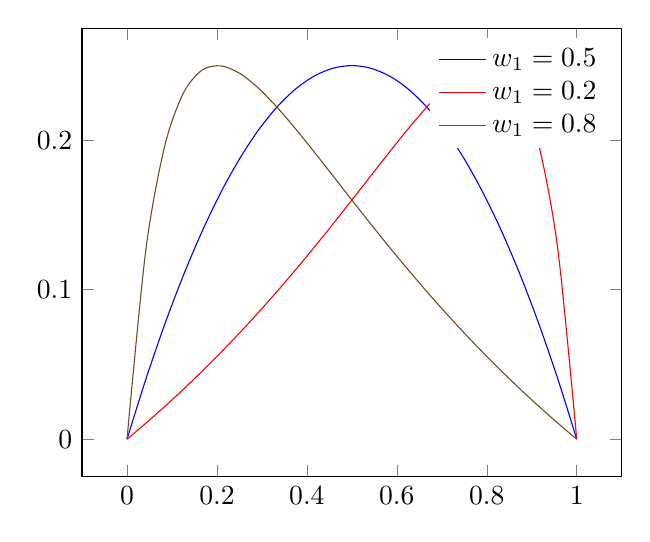
\begin{tikzpicture}
        \begin{axis}[domain=0:1, cycle list name=color, legend entries={$w_1=0.5$,$w_1=0.2$,$w_1=0.8$}, legend style={draw=none}]
            \addplot+[no markers, smooth] {0.5*x/(0.5*x+(1-0.5)*(1-x))*(1-0.5*x/(0.5*x+(1-0.5)*(1-x)))};
            \addplot+[no markers, smooth] {0.2*x/(0.2*x+(1-0.2)*(1-x))*(1-0.2*x/(0.2*x+(1-0.2)*(1-x)))};
            \addplot+[no markers, smooth] {0.8*x/(0.8*x+(1-0.8)*(1-x))*(1-0.8*x/(0.8*x+(1-0.8)*(1-x)))};
        \end{axis}
    \end{tikzpicture}
    \caption{Impuretés selon les poids relatifs}
\end{figure}

\begin{figure}[htbp]
    \begin{tikzpicture}
    \begin{axis}[domain=0:1, ymin=0, ymax = 1, enlargelimits = false, xlabel = {Taux de faux positifs}, ylabel = {Taux de vrais positifs}, legend style={draw=none,legend pos=south east}]
            \addplot[no markers, const plot, blue] table [x = "fpr", y = "tpr", col sep = comma] {images/roc_wrf.csv};
            \addlegendentry{WRF}
            \addplot[no markers, const plot] table [x = "fpr", y = "tpr", col sep = comma] {images/roc_rf.csv};
            \addlegendentry{RF}
            \addplot[no markers, black, dashed] {x};
    \end{axis}
    \end{tikzpicture}
    \caption{Performances de WRF ($\mathrm{AUC} = 0.8006$).}
\end{figure}

\subsection{Algorithme Metacost}

Une approche possible pour la création d'un algorithme d'apprentissage prenant en compte le coût est de modifier l'algorithme pour incorporer directement les coûts dans la construction, néanmoins cela reste une solution difficile à mettre en oeuvre et qu'il est nécessaire de répéter pour chaque algorithme que l'on veut adapter. Pour éviter ce travail long et fastidieux, \citet{PedroD} propose l'algorithme MetaCost qui permet de transformer tout algorithme qui peut fournir une approximation des probabilités de classification en un algorithme de minimisation des coûts.
Le but dans le cas de la minimisation du coût est de minimiser le risque conditionnel 
\begin{equation}
    R ( i \mid x ) = \sum_j \mathbb{P} ( j \mid x ) C(i,j) \label{idee_metacost}
\end{equation}
Cette règle partitionne l'espace $\mathcal{X}$ en $j$ régions de décision optimales. Notre but est alors de déterminer les frontières de ces espaces afin de construire notre classifieur. Il s'agit d'un problème difficile puisqu'il est possible que les étiquettes des individus d'apprentissage elles-mêmes ne soient pas optimales selon cette règle. L'idée de l'algorithme MetaCost est alors de réétiqueter l'échantillon d'apprentissage avec les classes optimales estimées et de réapprendre sur ce nouveau meta-échantillon.
Il faut tout d'abord un moyen d'estimer la probabilité conditionnelle d'appartenir à la classe $j$ de chaque individu d'apprentissage $x$, on utilise donc pour cela notre algorithme en lui-même. On peut ensuite calculer les nouvelles étiquettes optimales grâce à~\ref{idee_metacost}, réétiqueter l'échantillon d'apprentissage, et enfin apprendre notre classifieur final sur celui-ci.

Dans le cas des Forêts Aléatoires on possède déjà une bonne approximation des probabilités conditionnelles grâce à l'échantillon \ac{oob}. Il n'est donc pas nécessaire d'utiliser la procédure de Bagging, ici redondante, proposée par \citet{PedroD}. Dans les rares cas où $x$ n'est jamais \ac{oob}, on utilise comme approximation la probabilité issue de la forêt entière.

La procédure MetaCost pour les forêts aléatoires est résumée dans~\ref{alg:metacost}

\begin{algorithm}
\caption{Algorithme Metacost pour les forêts aléatoires}\label{alg:metacost}
\begin{algorithmic}
    \Procedure{Metacost-RF}{$S, C$}
    
    \State{ \texttt{RF} $\gets$ \texttt{ForêtsAléatoire(S)} }
    
    \For{ $(y,x) \in S$ }
        \For{ chaque classe $j$ }
            \If{$x \in \operatorname{OOB}(\texttt{RF})$}
                \State{ $\hat{p}(j \mid x) \gets \mathbb{P}_{\text{OOB}}(j \mid x)$ }
            \Else \State{$\hat{p}(j \mid x) \gets \texttt{RF}(j \mid x)$}
            \EndIf
        \EndFor
        \State{$y \gets \argmin_i \sum_j \hat{p}(j \mid x) C(i,j)$}
    \EndFor
    \State \Return $S$
    \EndProcedure
\end{algorithmic}    
\end{algorithm}

Dans le cadre des forêts aléatoires, le coût de la procédure n'est alors que deux fois plus élevé. Dans le cas où l'algorithme ne fournit pas de probabilités, il est toujours possible d'obtenir une approximation de celles-ci en procédant à un bagging comme dans le cas des forêts aléatoires, le coût est alors $N$ fois plus grand où $N$ est le nombre d'échantillons bootstrap construits.

\begin{figure}[htbp]
    \begin{tikzpicture}
    \begin{axis}[domain=0:1, ymin=0, ymax = 1, enlargelimits = false, xlabel = {Taux de faux positifs}, ylabel = {Taux de vrais positifs}, legend style={draw=none,legend pos=south east}]
            \addplot[no markers, const plot,blue] table [x = "fpr", y = "tpr", col sep = comma] {images/roc_mcrf.csv};
            \addlegendentry{RF+MC}
            \addplot[no markers, const plot] table [x = "fpr", y = "tpr", col sep = comma] {images/roc_rf.csv};
            \addlegendentry{RF}
            \addplot[no markers, black, dashed] {x};
    \end{axis}
    \end{tikzpicture}
    \caption{Performances de MetaCost + RF ($\mathrm{AUC} = 0.8217$).}
\end{figure}